\chapter{Cahier des charges}
% Partie dans laquelle on explique les features / requirements attendues
% On y trouve sans doute :

\epigraph{<< Les choses paraissent simples jusqu'à ce qu'on commence à les analyser >>}{Audrey Niffenegger}

\section{Analyse fonctionnelle}

\subsection*{Séparation des tâches}

Comme expliqué par les Echos\cite{SOD}, il s'agit  "d'un concept qui requière différents acteurs possédant des rôles et responsabilités différents pour la réalisation d’un ensemble de tâches dont l’exécution par un unique acteur pourrait potentiellement conduire à des fraudes ou des erreurs". \\


En effet, ce catalogue participatif nécessite un certain nombre de garde-fous afin de maintenir un outil qui dispose de ressources aussi bien de manière qualitative que quantitative. Notre analyse nous a permis d'isoler ces 4 types d'utilisateurs qui disposent de privilèges de manière incrémentale (en plus de disposer de leurs privilèges propres, chacun hérite aussi de ceux du précédent de la présente liste) :

\begin{itemize}
    \item Visiteur : Il s'agit d'un utilisateur non inscrit à notre plate-forme. Il ne peut rechercher et consulter que les fiches de ressources validés par un administrateur.
    \item Utilisateur : Il s'agit d'un utilisateur  inscrit à notre plate-forme. Celui-ci peut proposer des nouvelles ressources ainsi que de maintenir les fiches dont il est le créateur.
    \item Administrateur : Celui-ci crée/modifie des ressources de toute nature (fiches proposées par les utilisateurs, mots clés et catégories de mots clé), en plus de classifier les fiches.
    \item Super Administrateur : Celui-ci dispose du droit de supprimer de manière définitif les différentes ressources de notre plate-forme.
\end{itemize}

\pagebreak

\subsection*{État d'une fiche}

Au cours de notre analyse des processus de partage/modération de ressources informatiques, nous avons été confrontés à de nombreuses lacunes dans des systèmes similaires dont notamment :
\begin{itemize}
    \item Une manière unitaire/binaire de considérer les fiches. Il n'y a pas de nuance claire pour différencier la situation de celle-ci par rapport à une autre. Pour l'illustrer, prenons l'exemple d'une fiche qui est en cours de rédaction (et donc n'est pas encore prête à être publique) : bien souvent, cette information est absente.
    \item Le manque d'évolutivité dans la gestion des fiches. Conséquence du point précédent, cette lacune rend difficile l'ajout de nouvelles fonctionnalités telles que l'archivage numérique de ces ressources. 
\end{itemize}

C'est ainsi que nous avons décidé d'associer un état à chaque fiche, pour permettre de distinguer la situation de chacune au cours de ses processus. Le diagramme UML à états ci-dessous représente ces états et les principales transitions entre états (pour ne pas surcharger celui-ci) :

% width=\textwidth,height=\textheight,keepaspectratio
\begin{figure}[H]
    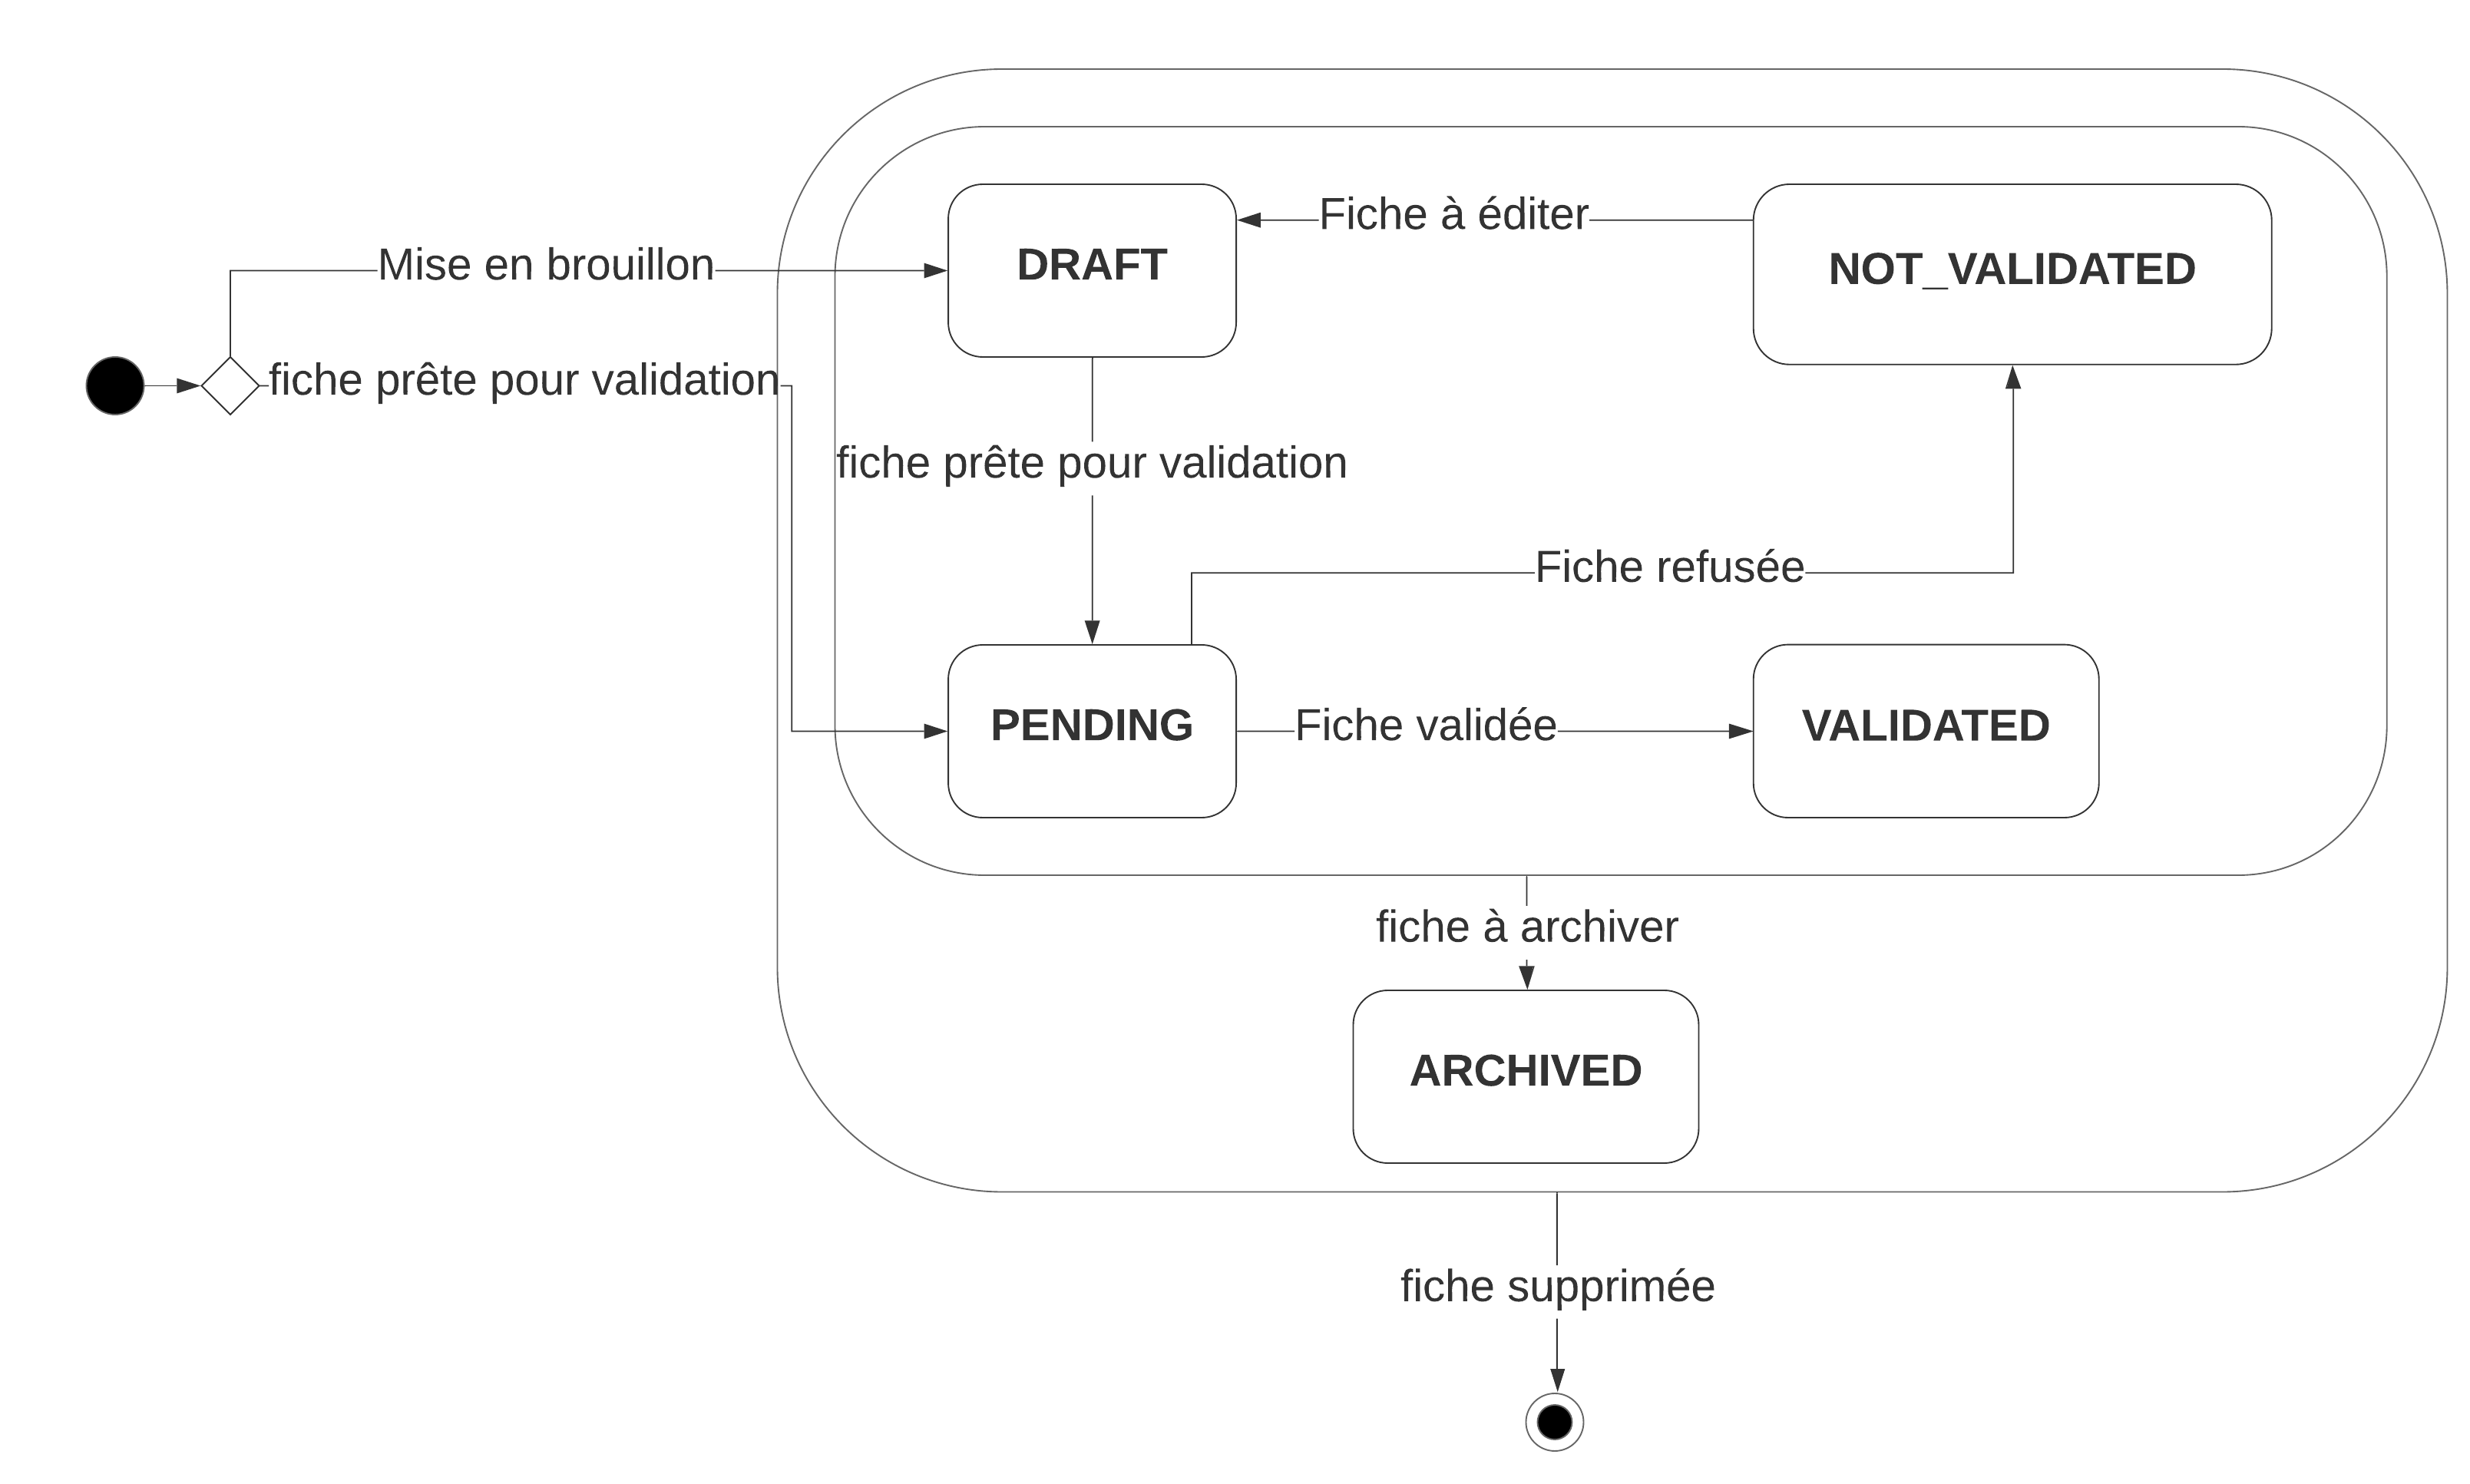
\includegraphics[width=\textwidth,height=\textheight,keepaspectratio]{images/StateFiches.png}
    \centering
    \caption{Diagramme UML à états pour l'état d'une fiche}
    \label{pic:stateDiagramForFiches}
\end{figure}

\subsection*{État des mots clés}

Une des questions annexes au sujet des fiches est la gestion des mots clés. En effet, les mots clés étant des éléments indispensables d'une fiche de qualité pour une meilleur référencement, il convient d'établir une stratégie précise pour exploiter au mieux ceux-ci. \\

Durant notre analyse, nous avons pu constater deux écoles de pensée bien distinctes (comparable à ce qui existe en économie) : 
\pagebreak
\begin{itemize}
    \item laissez-faire : Il s'agit de donner une liberté totale en matière de marquage (en utilisant aussi bien des mots clés existants que non). Bien que cette approche a le mérite de faire émerger de nouveaux mots clés par les contributions d'utilisateurs, cela restreint les possibilités de modération.
    \item l'interventionnisme : Il s'agit de restreindre le choix en matière de marquage (exclusivement des mots clés existants). Bien que cette approche rend la modération facile, cela restreint les possibilités de s'adapter à une réalité changeante.
\end{itemize}

Nous avons remarqué qu'aucune de ces deux possibilités ne se distinguait suffisamment de l'autre pour répondre de manière optimale à la problématique.
C'est pourquoi nous avons fait le choix d'une 3e voie, qui se situe donc entre ces 2 manières de penser. Tout comme les fiches, il s'agit d'ajouter un état à chaque mot clé pour distinguer sa situation propre. Le diagramme UML à états ci-dessous représente ces états et les principales transitions entre états (pour ne pas surcharger celui-ci) :

% width=\textwidth,height=\textheight,keepaspectratio
\begin{figure}[H]
    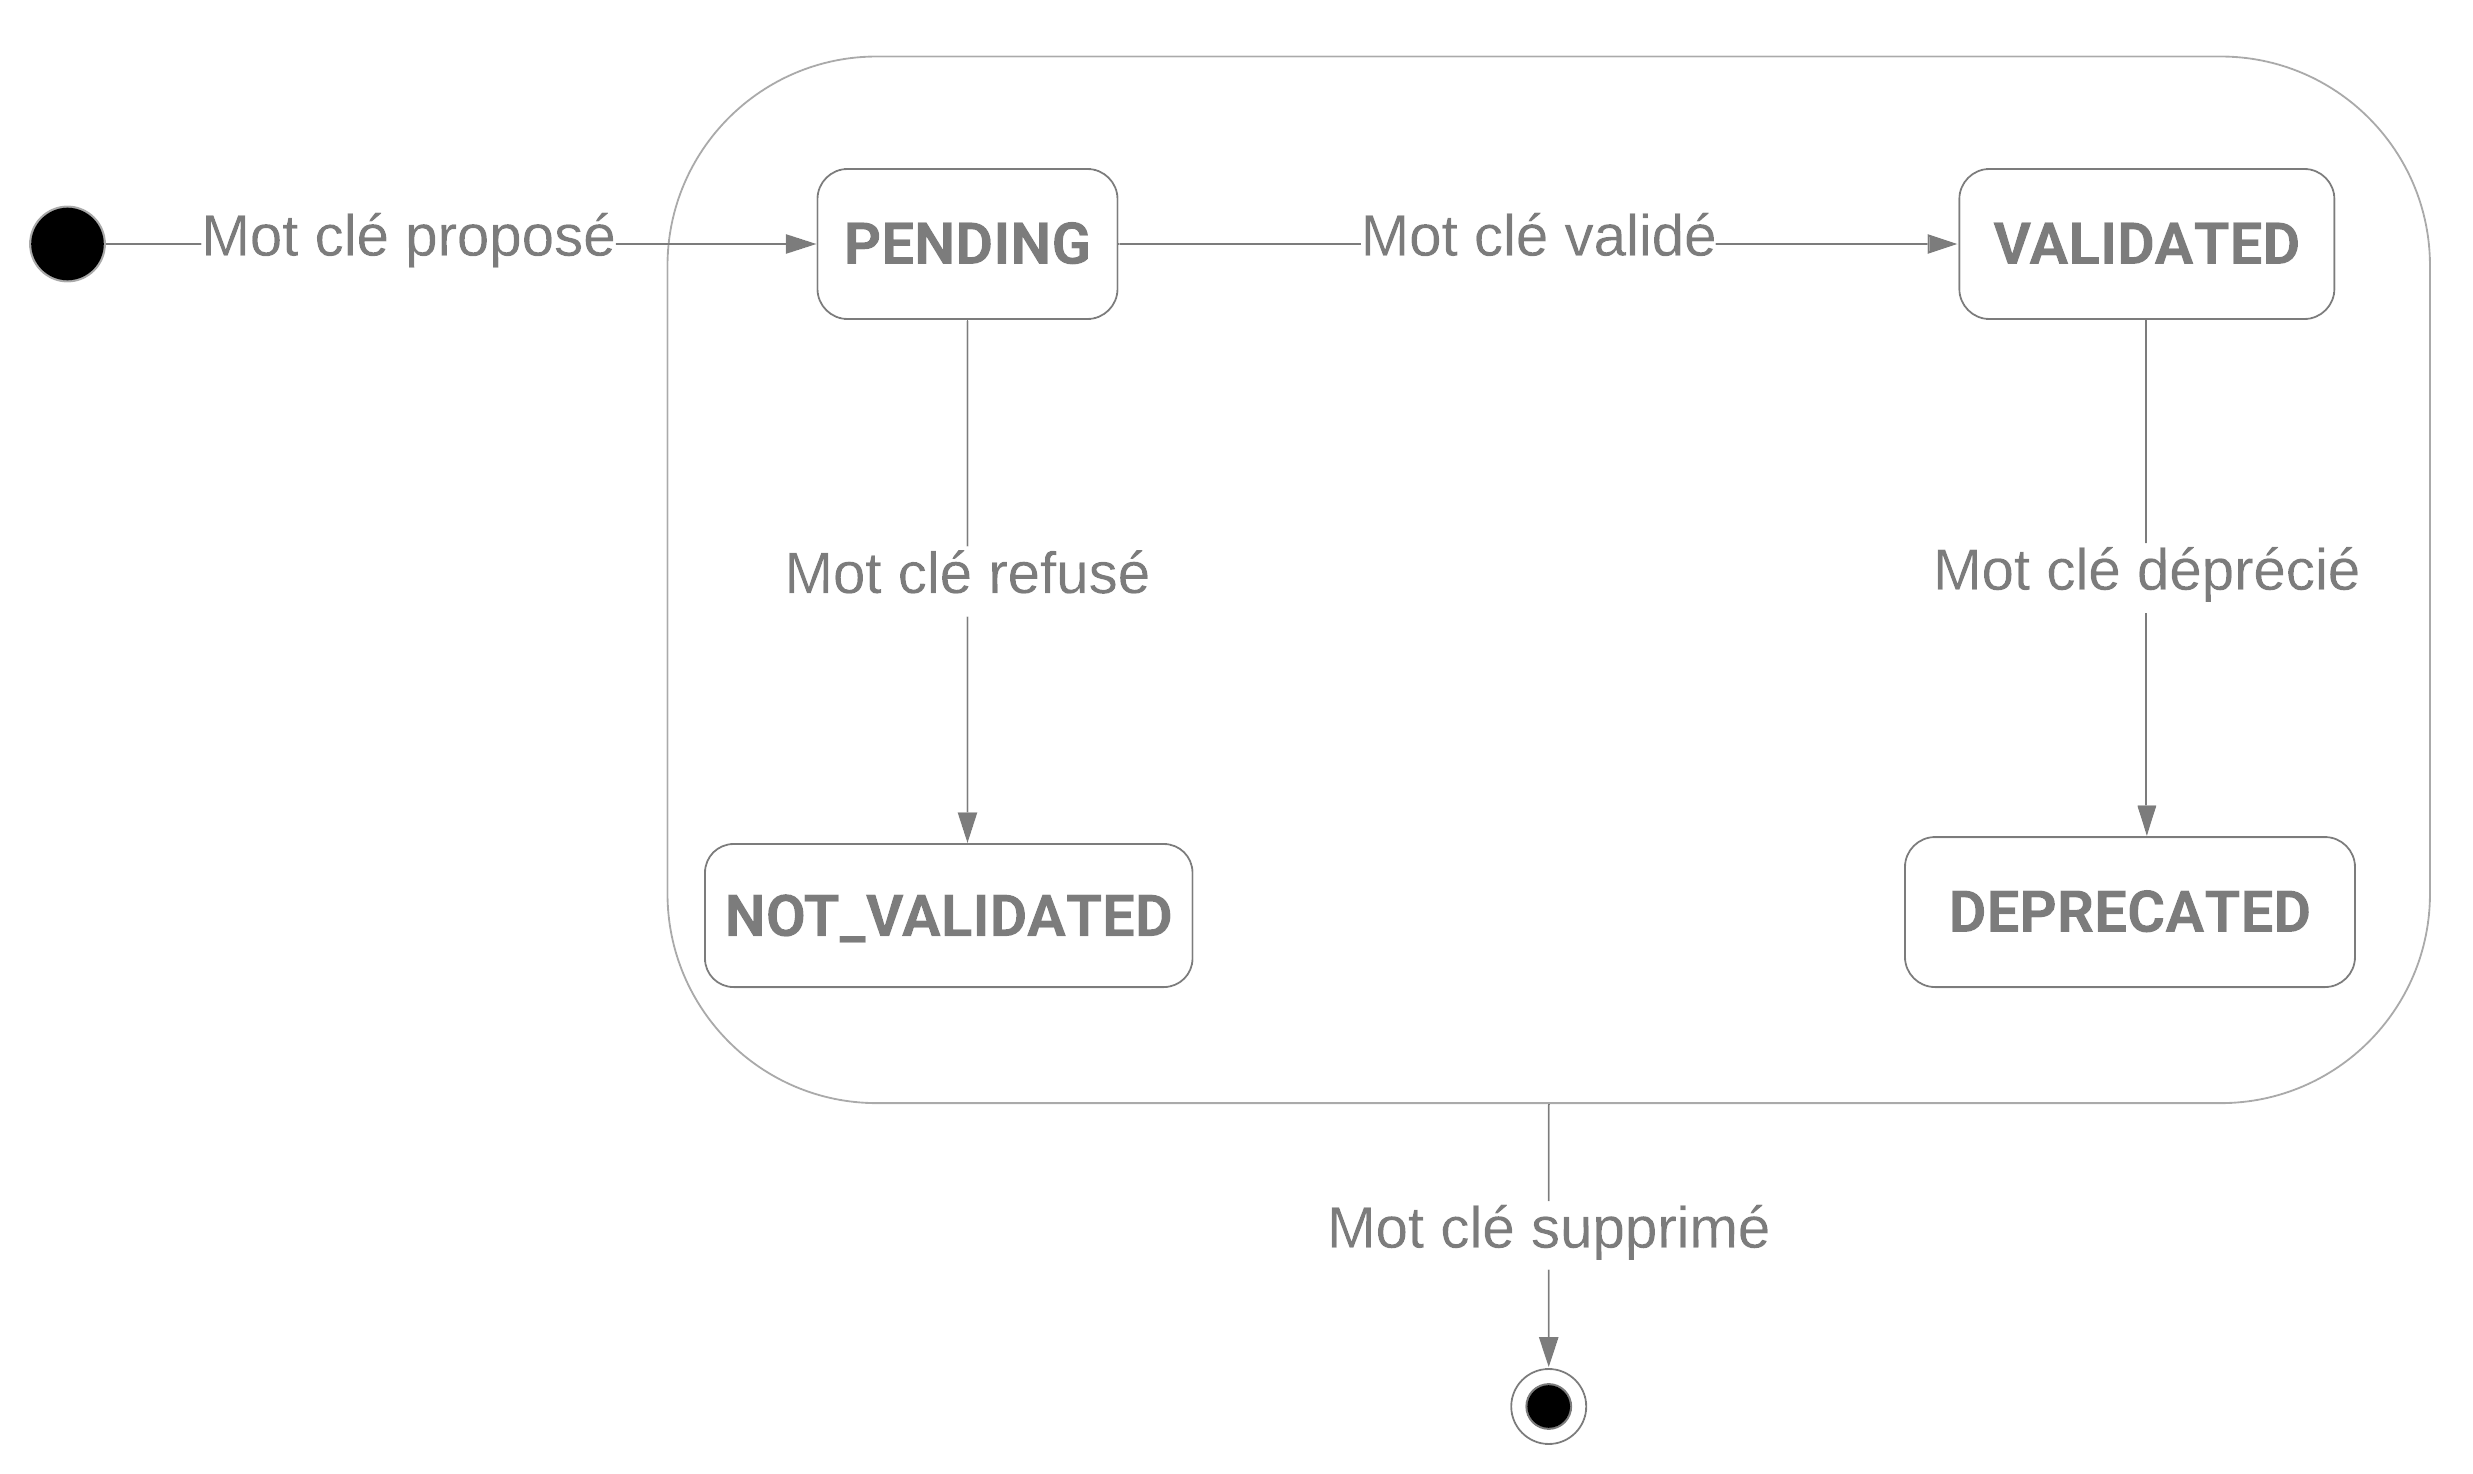
\includegraphics[width=\textwidth,height=\textheight,keepaspectratio]{images/StateTags.png}
    \centering
    \caption{Diagramme UML à états pour l'état d'un mot clé}
    \label{pic:stateDiagramForTags}
\end{figure}

\subsection*{Fonctionnalités}

TODO ( cela sera sans doute une liste de user stories , en fonction des utilisateurs )


% Image

% Users
% Exercise states
% Tag states
% Fonctionnalités 

% - diagrammes de cas d'utilisations ( + visuel qu'une liste de user stories )
% - explications des différents rôles dans l'application ( guest, user, admin )

\section{Analyse non-fonctionnelle}
% On explique ici ( design, ergonomie )
% Donner les critères d'ergonomie
% Pas forcément des tonnes de page : à priori 3-4 max devraient suffire

\section {Contraintes}
% Expliquer les contraintes :
%    - Maintenabilité / Extensibilité  du code
%    - Gestion simple du système ( quand Mens disait que les admins ne devaient pas avoir à toucher à la DB pour faire x ou y truc )
%    - Interface orienté vers l'UX ( une jolie instruction UI VS UX
%    - etc...